\section{Energy consumption}  
\label{sec:energetic}  
  
  
In order to analyse the energetic costs of the \ac{BLE} system implementation, a series of tests were designed and executed. The tests were divided into three categories: system off, system on and system working, presented in Section \ref{subsec:tests}.  
  
 
 
The used smartphone was a Sony Xperia E5, whose battery is rated at 2300 mAh. The battery values data collection was made through the android API, which allows one to know the battery percentage of the smartphone. This API allows one to obtain the current charge of a smartphone in terms of percentage, making it so that this condition imposes a constant error margin on the tests results.   
  
  
The tests were all conducted under the same base conditions, the battery was completely charged, without a SIM card and with the screen at maximum brightness. They were also conducted over the period of an hour.  
  
  
\subsection{Tests}  
\label{subsec:tests}  
  
  
\subsubsection{System Off}  
\label{subsec:sysoff}  
  
  
With this analysis one intends to understand the energetic cost of a smartphone on standby, i.e. idle and without service, in order to comprehend the baseline consumption and compare it with the energetic costs of the application, in multiple tests with varying factors.  
  
  
This category includes one single test case, case number 1, and its intention was to analyse the smartphone's energy consumption on standby with its sensors turned off. This case's test conditions were: having Wi-Fi and Bluetooth turned off and leaving the screen active on the main screen.  
  
  
\subsubsection{System On}  
\label{subsec:syson}  
  
  
In this category one will study the energetic impact of Wi-Fi and Bluetooth on the smartphone device. In order to do so, three tests were conducted: The first one (test case \#2, Wi-fi no service), activates the Wi-Fi without having available service; The second one (test case \#3 - wi-fi on), activates the Wi-Fi while providing service; and the last one (test case \#4 - system active), allows the same Wi-Fi conditions from the previous test (test case \#3) while activating Bluetooth.  
  
  
The last test, number 4, is fundamental, since it will allows for a better interpretation of the system's energy consumption. By providing a value for the energy consumption of the smartphone with everything active but the system, one can obtain more precisely the system operational costs.  
  
  
\subsubsection{System Working}  
\label{subsec:syswork}  
  
  
The system working category studies the energetic impact of the indoor location application on the smartphone. In order to do so, tests were conducted where two parameters were tuned, the number of nearby beacons and the discovery procedure frequency. The discovery period was tuned using four different values, five, fifteen, thirty and sixty seconds, while the number of nearby beacons was either one or two. Using all the possible parameters combinations, eight test cases were conducted.  
  
  
\subsubsection{Communication Costs}  
\label{subsec:commcosts}  
  
  
When proposing a generic architecture that is based on isolation of components in exchange for interoperability, it is important to analyse its drawbacks. In this case the isolation is obtained at the cost of higher communication costs, network communication with both the location and the maps server. In order to analyse the impact of this communication six test cases were used where two parameters were tuned: The number of nearby devices, one, two or three devices, and the operation that was carried out. While half of the tests performed the complete operational cycle, the remaining half didn't make use of any network communication, i.e. it completed the \ac{BLE} communication but stopped right after, before communication with any of the servers. This variations allows one to examine the amount of energy spent on network communications, while studying if there are noticeable differences relative to the number of nearby beacons. All the tests were made using a 5 second cycle period.  
  
  
  
  
\subsection{results}  
\label{subsec:results}  
  
  
\begin{itemize}  
  
\item The energetic cost's comparison of the three test cases for system on, as well as the one for system off can be seen on Figure \ref{fig:syson}.The presented figure allows one to visualize the overall energetic impact of the smartphone's sensors, which would be around 23 mAh, equivalent to one percent of the smartphone's battery. It is also possible to estimate that the Wi-fi sensor is the one contributing the most for this impact.   
It is important to keep the results of test case \#4 in mind, since it represents the energetic cost of having the smartphone application active alongside all of its required sensors, but without any of its functionalities active. This value in conjunction with the measures of the tests of the system working will allow to identify the costs of the application's functionalities .  
 
 
\begin{figure} [H] 
\centering  
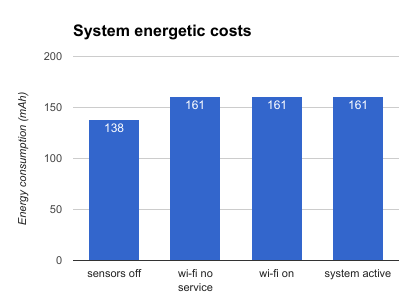
\includegraphics[width=0.5\linewidth]{5.Chapter/system-on.png}  
\caption[Test cases \#1-4: System On - energetic costs]{Test cases \#1-4: System On - energetic costs}  
\label{fig:syson}  
\end{figure}   
  
 
 
  
  
\item On Figure \ref{fig:syswork}, one can analyse the test cases from the system working group. Test case \#4 - system active is shown so that it is possible to better visualize the energetic cost of the application. The remaining data is grouped into pairs, with each pair having in common the used discovery procedure period. Test cases \#5 and \#6 use 5 seconds cycles, cases \#7 and \#8 use 15 seconds, cases \#9 and \#10 use 30 seconds and cases \#11 and \#12 use 60 seconds.  
  
\begin{figure}[H] 
\centering  
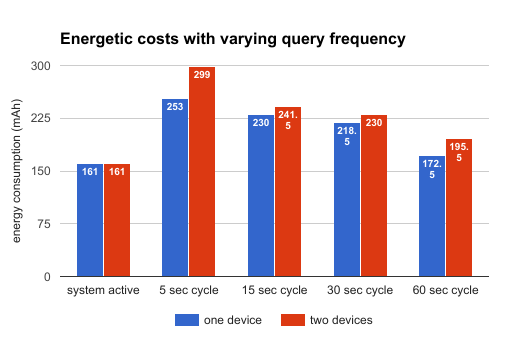
\includegraphics[width=0.5\linewidth]{5.Chapter/system-working.png}  
\caption[Test cases \#5-12: System Working - energetic costs]{Test cases \#5-12: System Working - energetic costs}  
\label{fig:syswork}  
\end{figure}  
  
From the figure, one can observe the energetic impact that occurs when adding an extra \ac{BLE} device for the application to interact with. The existence of more than one device leads to an energetic increase in the \ac{BLE} communication and as such the cost of this operation is proportionate to the number of existent nearby tags. When passing from one to two available devices, the number of operations is effectively doubled.  
  
Regarding the increase in cost associated to the number of beacons, the value here presented is highly increased due to the lack of optimisation. The insertion of a beacon cache, which although implemented wasn't used during testing, would reduce the cost of the \ac{BLE} communication operation to practically zero.  
The reason for this statement is that each beacon has a unique ID and, in a normal indoor environment, the user moves at low speed. Therefore the number of new beacons in each cycle is small. This situation leads to a beacon being heard multiple times, as such saving the server address associated to each beacon makes it so the \ac{BLE} communication query is required only once. By saving the information of the most recently contacted beacons, the number of required operations is proportional to the number of newly discovered beacons, instead of the number presented in these tests (equivalent to 1/2 new beacons in each cycle).  
  
  
  
 
 
  
  
\item Figure \ref{fig:commcost} presents the results for the communication cost analysis. It is possible to confirm that the network communication costs associated to the system are almost independent from the number of devices, having reached a flat cost of one percent of the phone battery in this case. This value can be interpreted according to the low amount of information that is being transmitted in each packet, i.e. each beacon's address and associated \ac{RSSI} value, that relative to the packet header isn't impactful when communicating with the location server.  The remaining messages are the answer from the location server to the smartphone, which has a constant small size (location information), and the messages to and from the maps server, which in this case is made through the google maps API and it is of relative constant size independently of the number of beacons.  
  
   
\begin{figure} [H] 
\centering  
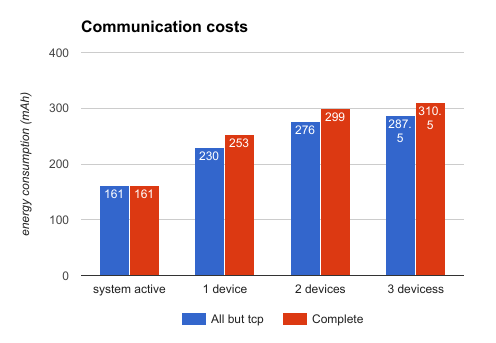
\includegraphics[width=0.5\linewidth]{5.Chapter/communication-costs.png}  
\caption[Communication's Energetic cost]{Communication's Energetic cost}  
\label{fig:commcost}  
\end{figure}  
  
  
\item Making use of the previously presented test cases, it is possible to obtain the average cost of network communication. The packet's average cost value and its intermediary values for calculation are present in Table \ref{table:packet}. Since the number of used packet during the test is capable of being calculated, the cost associated to each of them is also possible to calculate.   
  
\begin{table}[h!]  
\centering  
\begin{tabular}{ | m{5cm} | m{5cm} | }   
\hline  
Nº cycles / 1 hour &  720 \\   
\hline  
Nº packets / cycle & 4 \\   
\hline  
Communication Cost & 23 mAh \\   
\hline  
Average packet cost & 0.008 mAh ( 1/2880\% ) \\   
\hline  
\end{tabular}  
\caption[Packet's average cost]{Packet's average cost}  
\label{table:packet}  
\end{table}  
 
 
Overall the added cost caused by externalising both the maps and the location component into servers is low. This energetic impact is still not representative of the actual network communication cost of a real system deployed according to the proposed generic framework since there are optimizations that aren't being taken into consideration. An example of an optimisation, would be achieved through the usage of the accelerometer or any other sensor capable of detecting user movement. When capable of detection such event, the system would avoid requesting the user's location until movement occurs. This optimisation would be capable of reducing the overall system consumption. 
\end{itemize}  
  
 